\documentclass{article}\usepackage{graphicx, color}
%% maxwidth is the original width if it is less than linewidth
%% otherwise use linewidth (to make sure the graphics do not exceed the margin)
\makeatletter
\def\maxwidth{ %
  \ifdim\Gin@nat@width>\linewidth
    \linewidth
  \else
    \Gin@nat@width
  \fi
}
\makeatother

\definecolor{fgcolor}{rgb}{0.2, 0.2, 0.2}
\newcommand{\hlnumber}[1]{\textcolor[rgb]{0,0,0}{#1}}%
\newcommand{\hlfunctioncall}[1]{\textcolor[rgb]{0.501960784313725,0,0.329411764705882}{\textbf{#1}}}%
\newcommand{\hlstring}[1]{\textcolor[rgb]{0.6,0.6,1}{#1}}%
\newcommand{\hlkeyword}[1]{\textcolor[rgb]{0,0,0}{\textbf{#1}}}%
\newcommand{\hlargument}[1]{\textcolor[rgb]{0.690196078431373,0.250980392156863,0.0196078431372549}{#1}}%
\newcommand{\hlcomment}[1]{\textcolor[rgb]{0.180392156862745,0.6,0.341176470588235}{#1}}%
\newcommand{\hlroxygencomment}[1]{\textcolor[rgb]{0.43921568627451,0.47843137254902,0.701960784313725}{#1}}%
\newcommand{\hlformalargs}[1]{\textcolor[rgb]{0.690196078431373,0.250980392156863,0.0196078431372549}{#1}}%
\newcommand{\hleqformalargs}[1]{\textcolor[rgb]{0.690196078431373,0.250980392156863,0.0196078431372549}{#1}}%
\newcommand{\hlassignement}[1]{\textcolor[rgb]{0,0,0}{\textbf{#1}}}%
\newcommand{\hlpackage}[1]{\textcolor[rgb]{0.588235294117647,0.709803921568627,0.145098039215686}{#1}}%
\newcommand{\hlslot}[1]{\textit{#1}}%
\newcommand{\hlsymbol}[1]{\textcolor[rgb]{0,0,0}{#1}}%
\newcommand{\hlprompt}[1]{\textcolor[rgb]{0.2,0.2,0.2}{#1}}%

\usepackage{framed}
\makeatletter
\newenvironment{kframe}{%
 \def\at@end@of@kframe{}%
 \ifinner\ifhmode%
  \def\at@end@of@kframe{\end{minipage}}%
  \begin{minipage}{\columnwidth}%
 \fi\fi%
 \def\FrameCommand##1{\hskip\@totalleftmargin \hskip-\fboxsep
 \colorbox{shadecolor}{##1}\hskip-\fboxsep
     % There is no \\@totalrightmargin, so:
     \hskip-\linewidth \hskip-\@totalleftmargin \hskip\columnwidth}%
 \MakeFramed {\advance\hsize-\width
   \@totalleftmargin\z@ \linewidth\hsize
   \@setminipage}}%
 {\par\unskip\endMakeFramed%
 \at@end@of@kframe}
\makeatother

\definecolor{shadecolor}{rgb}{.97, .97, .97}
\definecolor{messagecolor}{rgb}{0, 0, 0}
\definecolor{warningcolor}{rgb}{1, 0, 1}
\definecolor{errorcolor}{rgb}{1, 0, 0}
\newenvironment{knitrout}{}{} % an empty environment to be redefined in TeX

\usepackage{alltt}
\usepackage{amsmath}
\IfFileExists{upquote.sty}{\usepackage{upquote}}{}
\begin{document}
\title{London R Practice}
\author{Rob Hayward}
\maketitle
\section{Introduction}

This is a file to run through the presentation that was made at the September 2013 London R by Maarten Speekenbrink.  

I am not sure how to load the appropriate packages (so this can probably be deleted in the future).  However, I will do that in a chunk. The information is in the title:  dependent mixed models. This is to implement micture and hidden Markov models. 


\section{Mixed Models}
From the London R presentation. In a \emph{mixture model} each observation is assumed to be drawn from a number of distinct subpopulation (``component distributions'' according to Maarten).  The distribution from which the observation is drawn is not directly observable and therefore it is represented by a \emph{latent state}.  

A mixture distribution is defined as 
\begin{equation}
p(Y_1 = y) = \sum_{i - 1}^N p(Y_t = y|S_t = i)P(S_t = i)
\end{equation}
where,
\begin{itemize}
\item $S_t \in {1, \dots, N}$ denotes the latent state or class of observation t
\item $P(S_t = i)$ denots the probability of the latent state t equals i 
\item $p(Y_t = y|S_t = i)$ denotes the density of observation of $Y_t$ conditional on latent state being $S_t = i$.
\end{itemize}
\section{Perth Water Example}

\section{Change Model}
This is a model that assumes one or more discrete change points in the data. It may be the mean, trend or other parameters that may change. In this example with the S\&P 500 it is the mean and the standard deviation. There is a transition matrix that defines the change points.  For example, if there is one transition the matrix would be along the lines of 
\begin{equation*}
\begin{pmatrix}
p_1 & 1 - p_1 \\
0 & 1
\end{pmatrix}
\end{equation*}
Where $p_1$ is the probability that the system will be in state 1.  One there is a switch to state two.  This matrix can be extended for more states. Need to come back and look at this if I can get the data. 

\section{S\&P 500 Example}
\begin{knitrout}
\definecolor{shadecolor}{rgb}{0.969, 0.969, 0.969}\color{fgcolor}\begin{kframe}
\begin{alltt}
\hlfunctioncall{library}(TTR)
\hlcomment{# load SP500 returns}
\hlfunctioncall{Sys.setenv}(tz = \hlstring{"UTC"})
sp500 <- \hlfunctioncall{getYahooData}(\hlstring{"^GSPC"}, start = 19500101, end = 20120909, freq = \hlstring{"daily"})
ep <- \hlfunctioncall{endpoints}(sp500, on = \hlstring{"months"}, k = 1)
sp500 <- sp500[ep[2:(\hlfunctioncall{length}(ep) - 1)]]
sp500$logret <- \hlfunctioncall{log}(sp500$Close) - \hlfunctioncall{lag}(\hlfunctioncall{log}(sp500$Close))
sp500 <- \hlfunctioncall{na.exclude}(sp500)
\end{alltt}
\end{kframe}
\end{knitrout}

Now plot the data to get an idea of what it looks like. 
\begin{knitrout}
\definecolor{shadecolor}{rgb}{0.969, 0.969, 0.969}\color{fgcolor}\begin{kframe}
\begin{alltt}
\hlfunctioncall{plot}(sp500$logret, main = \hlstring{"S&P 500 log returns"})
\end{alltt}
\end{kframe}
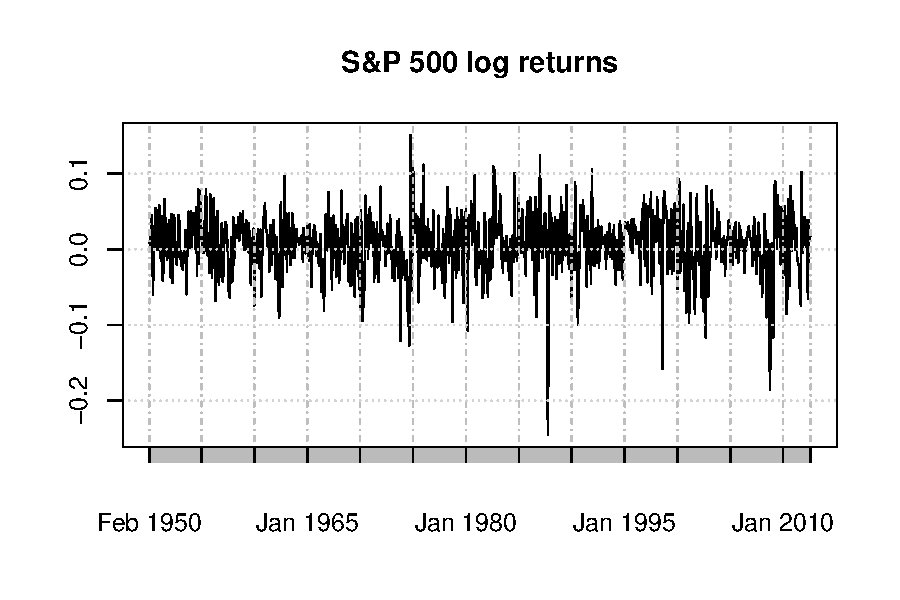
\includegraphics[width=\maxwidth]{figure/plot} 

\end{knitrout}

The aim is to identify the bull and bear markets. First set up the model (mod). This is a logistic regression ("logret") with two states. Then fit the model.   
\begin{knitrout}
\definecolor{shadecolor}{rgb}{0.969, 0.969, 0.969}\color{fgcolor}\begin{kframe}
\begin{alltt}
mod <- \hlfunctioncall{depmix}(logret ~ 1, nstates = 2, data = sp500)
\hlfunctioncall{set.seed}(1)
fm2 <- \hlfunctioncall{fit}(mod, verbose = FALSE)
\end{alltt}
\begin{verbatim}
## iteration 88 logLik: 1348
\end{verbatim}
\end{kframe}
\end{knitrout}

The number of iterations and the log likelihood is printed.  Now summarise the information. 
\begin{knitrout}
\definecolor{shadecolor}{rgb}{0.969, 0.969, 0.969}\color{fgcolor}\begin{kframe}
\begin{alltt}
depmixS4::\hlfunctioncall{summary}(fm2)
\end{alltt}
\begin{verbatim}
## Initial state probabilties model 
## Model of type multinomial (identity), formula: ~1
## <environment: 0x000000001202e608>
## Coefficients: 
##           [,1] [,2]
## [1,] 1.735e-47    1
## 
## Transition model for state (component) 1 
## Model of type multinomial (identity), formula: ~1
## <environment: 0x0000000011a4ccb8>
## Coefficients: 
## [1] 0.8215 0.1785
## 
## Transition model for state (component) 2 
## Model of type multinomial (identity), formula: ~1
## <environment: 0x0000000011a4ccb8>
## Coefficients: 
## [1] 0.03914 0.96086
## 
## 
## Response model(s) for state 1 
## 
## Response model for response 1 
## Model of type gaussian (identity), formula: logret ~ 1
## Coefficients: 
## [1] -0.01505
## sd  0.06484 
## 
## 
## Response model(s) for state 2 
## 
## Response model for response 1 
## Model of type gaussian (identity), formula: logret ~ 1
## Coefficients: 
## [1] 0.01045
## sd  0.03378
\end{verbatim}
\end{kframe}
\end{knitrout}



\end{document}
